\section{Results}
\label{sec:results}

We present results in three parts: the cross-domain comparison with cross-family validation (Section~\ref{sec:cross_domain}), the counterfactual ablation (Section~\ref{sec:counterfactual}), and the finance-specific failure taxonomy (summarized here, detailed in Section~\ref{sec:finance_challenges}).

\subsection{Cross-Domain Comparison}
\label{sec:cross_domain}

We ran five parsers on four mathematical benchmarks (GSM8K, SVAMP, ASDiv, MultiArith) and two financial benchmarks (FinQA, FLARE-FinQA), using Qwen3-1.7B and 8B across all benchmarks, with GLM-4-9B-Chat on the financial benchmarks for cross-family validation.

Table~\ref{tab:cross_domain} presents the complete cross-domain comparison. We report two metrics: the \textbf{full spread} (best $-$ worst overall) and the \textbf{Res-A spread} (difference among the four parsers excluding \numparser{}). Res-A includes the potentially format-specific \boxedparser{} parser, so it can still reflect \LaTeX{} output conventions. To assess whether residual sensitivity persists among parsers that are truly format-compatible for most model outputs, we additionally report \textbf{Res-B spread} (excluding both \numparser{} and \boxedparser{}, comparing only \texttt{fixed}, \texttt{last\_number}, and \texttt{finance\_aware}) in the text where informative. Full parser-level results including both metrics are available in our released data.

\begin{table}[htb!]
\caption{Cross-domain parser sensitivity: accuracy (\%) of five parsers across four mathematical and two financial benchmarks. Res-A = max $-$ min among boxed, fixed, last, fin\_aware; Res-B = max $-$ min among fixed, last, fin\_aware only. \emph{Italicized} = cross-family GLM.}
\label{tab:cross_domain}
\centering
\resizebox{\columnwidth}{!}{%
\begin{tabular}{@{}lllrrrrrrr@{}}
\toprule
Domain & Benchmark & Model & eq & boxed & fixed & last & fin\_aware & Res-A & Res-B \\
\midrule
\multirow{4}{*}{Math} & \multirow{2}{*}{MultiArith} & 1.7B & 16 & 96 & 97 & 97 & 96 & 1 & 1 \\
& & 8B  & 12 & 95 & 100 & 99 & 100 & 5 & 1 \\
\cmidrule{3-10}
& \multirow{2}{*}{SVAMP} & 1.7B & 33 & 91 & 92 & 90 & 92 & 2 & 2 \\
& & 8B  & 27 & 87 & 92 & 88 & 93 & 6 & 5 \\
\cmidrule{3-10}
& \multirow{2}{*}{ASDiv} & 1.7B & 31 & 92 & 93 & 91 & 92 & 2 & 2 \\
& & 8B  & 37 & 94 & 95 & 91 & 94 & 4 & 4 \\
\cmidrule{3-10}
& \multirow{2}{*}{GSM8K} & 1.7B & 10 & 81 & 82 & 80 & 87 & 7 & 7 \\
& & 8B  & 8 & 94 & 95 & 90 & 95 & 5 & 5 \\
\midrule
\multirow{6}{*}{Fin.} & \multirow{3}{*}{FinQA} & 1.7B & 12 & 28 & 34 & 38 & 35 & 10 & 4 \\
& & 8B  & 11 & 12 & 25 & 44 & 28 & 32 & 19 \\
& & \emph{GLM} & \emph{9} & \emph{0.0} & \emph{41} & \emph{49} & \emph{42} & \emph{49} & \emph{8} \\
\cmidrule{3-10}
& \multirow{3}{*}{FLARE} & 1.7B & 14 & 12 & 30 & 25 & 24 & 18 & 6 \\
& & 8B  & 14 & 6 & 19 & 22 & 20 & 16 & 3 \\
& & \emph{GLM} & \emph{13} & \emph{0.0} & \emph{29} & \emph{19} & \emph{24} & \emph{29} & \emph{10} \\
\bottomrule
\end{tabular}%
}
\end{table}

\begin{figure}[htb!]
\centering
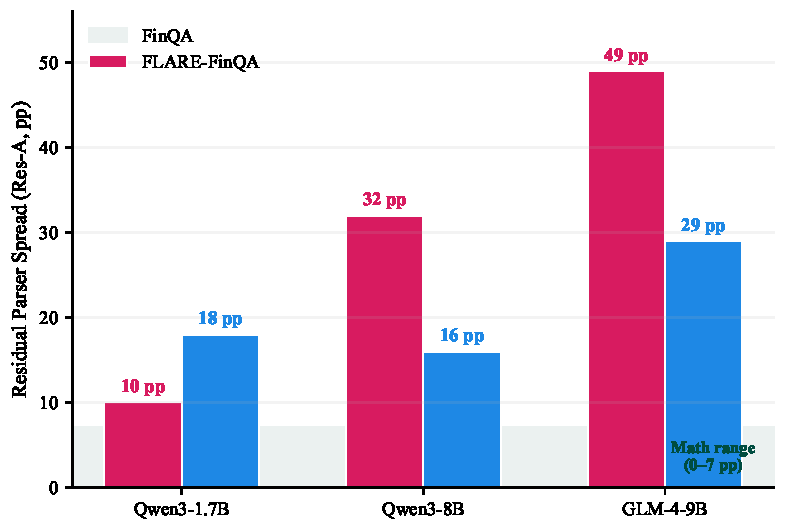
\includegraphics[width=\columnwidth]{figures/figure2_residual_scale.pdf}
\caption{Residual parser spread (Res-A) across models. FinQA spread increases from 10\,pp (Qwen3-1.7B) to 32\,pp (Qwen3-8B); GLM-4-9B (cross-family) reaches 49\,pp. FLARE-FinQA spans 16--29\,pp. The shaded band (0--7\,pp) marks the range observed across all mathematical benchmarks.}
\label{fig:residual_scale}
\end{figure}

Two layers are visible in Table~\ref{tab:cross_domain}. \textbf{Layer~1: the \numparser{} parser fails on every benchmark.} The full spread---max $-$ min across all five parsers---ranges from 16\pp{} (FLARE 8B) to 87\pp{} (GSM8K 8B) across all conditions. The largest gap occurs on a mathematical benchmark, not a financial one. Format mismatch between parser assumption and model output convention is a universal evaluation problem.

\textbf{Layer~2: residual sensitivity differs by domain.} The primary metric is Res-B (excluding both \numparser{} and \boxedparser{}): financial benchmarks show 3--19\pp{}, versus 1--7\pp{} on mathematical controls. Res-A (excluding only \numparser{}) ranges from 10--49\pp{}, but it includes the potentially format-specific \boxedparser{} parser and is inflated by \boxedparser{} incompatibility---GLM scores 0\% on \boxedparser{}, which alone contributes 49\pp{} of that range. On math, once the format is correctly handled, all reasonable parsers agree within single-digit percentages (1--7\pp{} under both Res-A and Res-B). On finance, parser choice continues to move accuracy substantially, though the degree varies by benchmark and residual definition.

\begin{figure}[htb!]
\centering
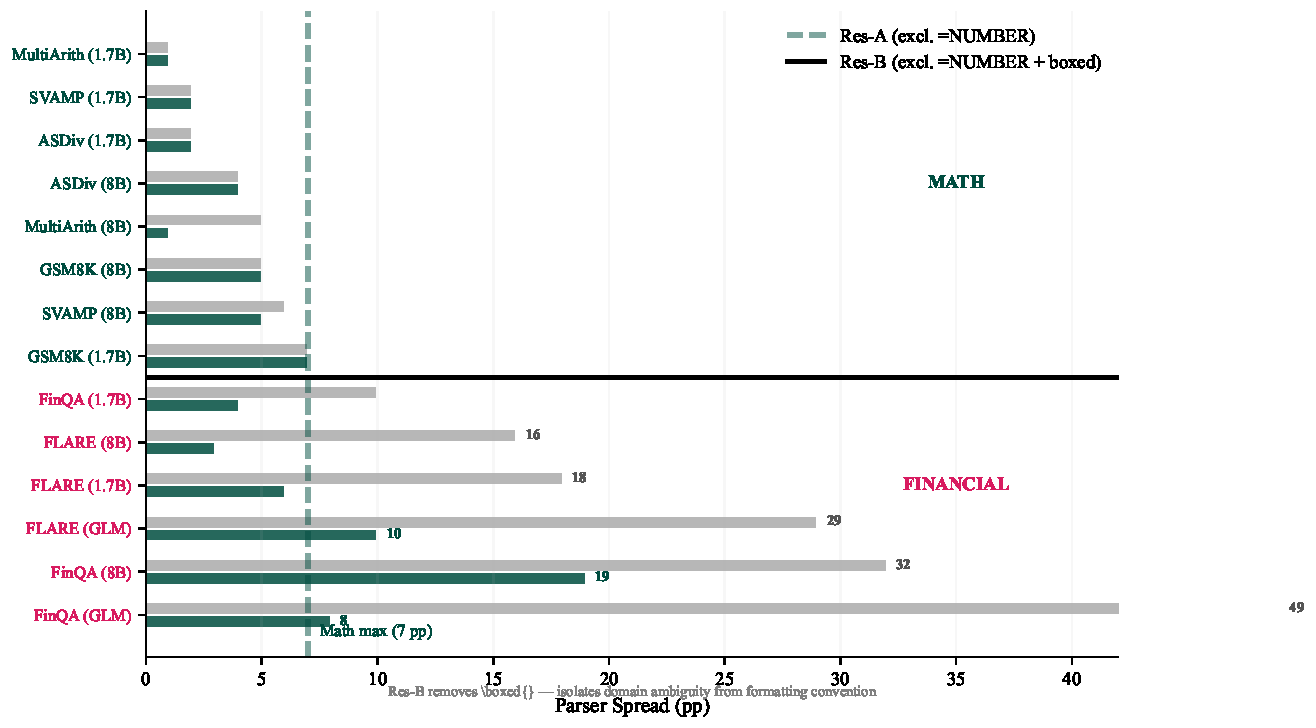
\includegraphics[width=\columnwidth]{figures/figure4_resA_resB.pdf}
\caption{Res-A versus Res-B: isolating domain-level parser sensitivity from format-convention effects. Light gray bars show Res-A (excluding only \numparser{}); dark green bars show Res-B (excluding both \numparser{} and \boxedparser{}). Financial benchmarks retain elevated sensitivity under Res-B on the largest-effect conditions (FinQA 8B at 19\,pp, FLARE GLM at 10\,pp). Some financial conditions narrow to math-like levels under Res-B (FLARE 8B 3\,pp, FinQA GLM 8\,pp).}
\label{fig:resAB}
\end{figure}

Table~\ref{tab:cross_domain} also reports \textbf{Res-B} (excluding both \numparser{} and \boxedparser{}), which isolates domain-level ambiguity from format-convention effects. Under Res-B, financial spreads narrow but remain elevated on the largest-effect conditions (FinQA 8B at 19\,pp, FLARE GLM at 10\,pp). Some financial conditions narrow to math-like levels (FLARE 8B 3\,pp, FinQA GLM 8\,pp), suggesting partial format-driven sensitivity. The core finding holds: on FinQA 8B (19\,pp Res-B), the effect survives removing \boxedparser{}.

\textbf{Scale and cross-family effects.} On FinQA, the residual spread increases from 10\pp{} (Qwen3-1.7B) to 32\pp{} (Qwen3-8B), and reaches 49\pp{} for the cross-family GLM-4-9B model. This pattern---the effect is not specific to a single architecture ---is corroborated on FLARE-FinQA (18\pp{}, 16\pp{}, 29\pp{} for 1.7B, 8B, GLM).

\textbf{Sampling uncertainty.} We bootstrap 95\% confidence intervals for Res-A and Res-B spreads over benchmark items (10K resamples). For Res-A, FinQA 8B yields 32.0\,pp CI~[23.0,\,42.0] versus GSM8K 8B 5.0\,pp CI~[1.0,\,10.0]; the CIs do not overlap. FinQA 1.7B (10.0\,pp, CI~[4.0,\,17.0]) overlaps with GSM8K 1.7B (7.0\,pp, CI~[2.0,\,12.0]). For Res-B, FinQA 8B yields 19.0\,pp CI~[11.0,\,27.0] versus GSM8K 8B 5.0\,pp CI~[1.0,\,10.0]; again the CIs do not overlap. FinQA 1.7B (4.0\,pp, CI~[1.0,\,10.0]) and GSM8K 1.7B (7.0\,pp, [2.0,\,12.0]) overlap substantially with no significant difference.

To directly test whether the Res-B gap between financial and mathematical benchmarks is significant, we compute the bootstrap distribution of the difference between independent two-sample resamples (FinQA $-$ GSM8K, 10K iterations). For the 8B models, the difference is 14.1\,pp, 95\% CI~[5.0,\,23.0]\,pp, which excludes zero ($p = 0.001$). For the 1.7B models, the difference is $-2.5$\,pp, CI~[$-$9.0,\,5.0]\,pp, not significant ($p = 0.77$). The Res-A difference is also significant for 8B (26.9\,pp, CI~[16.0,\,38.0]\,pp) but not for 1.7B. Thus the sensitivity difference between FinQA and GSM8K is statistically robust at the 8B scale for both residual definitions; the 1.7B models, with lower baseline accuracy, do not show a significant domain gap.

\textbf{Oracle upper bound.} We compute the oracle accuracy achievable by multi-parser aggregation: an answer is counted correct if \emph{any} of the five parsers extracts the correct answer. The oracle improves over the best single parser by only 1--2\,pp on FinQA and 0--1.0\,pp on GSM8K. While parser choice materially affects measured accuracy, parser ensembling alone cannot close the main performance gap; 47--58\% of FinQA items are missed by all five parsers simultaneously, confirming that model reasoning capability, not extraction method, is the dominant absolute bottleneck on these benchmarks.

\textbf{No single parser is optimal across financial benchmarks.} On FinQA, \texttt{last\_number} wins by substantial margins in all model conditions. On FLARE-FinQA, \texttt{fixed} wins on 1.7B and GLM, while \texttt{last\_number} wins on 8B. These benchmarks both target financial numerical reasoning, yet their optimal extraction strategies differ. There is no single correct parser for financial evaluation; multi-parser evaluation should become standard practice.

\textbf{Parser choice changes who wins.} We compute rank correlations (Kendall $\tau$) between parser-induced model orderings. On FinQA, the winner changes from Qwen3-1.7B under \numparser{} and \boxedparser{} to GLM-4-9B under the other three parsers---a complete reversal of the top-ranked model. The extreme case is \numparser{} vs.\ \texttt{last\_number}: $\tau = -1.00$ (Spearman $\rho = -1.00$), meaning the model ranking is perfectly inverted (all three model pairs swap order). Even among the three reasonable parsers, \texttt{fixed} vs.\ \texttt{last\_number} has $\tau = +0.33$ ($\rho = +0.50$) with 1 of 3 model pairs reversing order, while \texttt{fixed} and \texttt{finance\_aware} agree perfectly ($\tau = +1.00$). On FLARE-FinQA, rankings are more stable: Qwen3-1.7B is top-ranked or tied under all five parsers, and pairwise $\tau$ ranges from +0.33 to +1.00 with at most 1 reversal per pair. This asymmetry---FinQA rankings are parser-sensitive, FLARE rankings are more robust---is itself evidence that benchmark design choices affect extraction sensitivity.

\textbf{Cross-family validation.} To confirm that extraction sensitivity is not specific to the Qwen3 architecture, we evaluated GLM-4-9B-Chat~\cite{glm2024} on both financial benchmarks. GLM reproduces the qualitative pattern: its Res-A spread reaches 49\,pp on FinQA, the largest value observed. Under Res-B (excluding \boxedparser{}, which scores 0\% because GLM never uses \LaTeX{} formatting), the spreads are 8\,pp and 10\,pp---still comparable to or larger than the math range. This confirms that \boxedparser{} extraction depends on model-specific output conventions, and that cross-family validation must account for format compatibility.

\subsection{Matched Counterfactual: Stripping Financial Surface Forms}
\label{sec:counterfactual}

To isolate the role of financial surface forms from output-format conventions, we run a counterfactual ablation: we take the model outputs for FinQA 8B and FLARE 8B, strip all financial formatting (currencies, percentages, magnitudes, accounting negatives) from the response text, and re-apply the same five parsers. If financial formats are what make the parsers disagree, stripping them should narrow the Res-B gap; if a domain-aware parser was using those formats correctly, stripping them can instead increase disagreement by removing that advantage.

On FinQA 8B, the Res-B gap narrows from 19.0\,pp to 11.0\,pp after stripping, with 14 of 500 extraction decisions changing. Financial surface forms account for approximately 8\,pp of the 19\,pp gap, while the remaining 11\,pp persists after stripping. Combined with the supplementary audit of Res-B disagreements (Section~\ref{sec:finance_challenges}), the residual 11\,pp is driven by output-level conventions---multi-step extraction position, gold-answer normalization, and sign formatting---rather than the \boxedparser{}-style format mismatch that inflates Res-A.

On FLARE 8B, the opposite occurs: Res-B \emph{increases} from 3.0\,pp to 10.0\,pp after stripping. The mechanism is that \texttt{finance\_aware} correctly interprets financial surface forms in the original outputs, and stripping them removes its advantage, causing it to disagree more with the other parsers. This asymmetry---FinQA sensitivity is driven by output-level conventions, while FLARE exposes the benefit of finance-aware normalization---explains why the two benchmarks show different residual spread profiles and confirms that domain-aware parsing matters when outputs contain financial formats.

\subsection{Finance-Specific Failure Taxonomy}

We conducted a manual audit of 104 model responses on FinQA, classifying extraction failures into six categories: format mismatch (40\%), magnitude confusion (15\%), multi-step extraction (15\%), currency prefix stripping (12\%), percentage normalization (10\%), and sign convention errors (8\%). Full details including annotation protocol, inter-annotator agreement, and per-category examples are in Section~\ref{sec:finance_challenges}. The four finance-specific categories (magnitude, currency, percentage, sign) account for 45\% of failures. Combined with the cross-domain comparison, these categories explain why financial benchmarks retain elevated residual sensitivity even after format mismatch is controlled: parsers must handle domain-specific numeric conventions that do not appear in standard math problems.
